\section{Thursday, March 13: Support Vector Machines}

Like Monday's class, today's class might at first seem like we are just randomly jumping to a new algorithm. But I hope that by the end of class, you are once again motivated to think of this instead as a new lens through which to study our important themes from the class. Today's theme is all about feature engineering in a really clever way, and what that gets us. SVMs also have some historical importance! 

\subsection{Motivation for SVMs}

To motivate today's class, we are going to be thinking about a picture that we haven't thought about since the day that we covered LDA. The picture is of two quantitative predictors $X_1$ and $X_2$, and a categorical response $y$ (shown by the colors). See Figure~\ref{fig_svm}.

Consider the left panel of Figure~\ref{fig_svm}. Our goal is to predict $Y$ using $X_1$ and $X_2$. In this case, the tasks looks almost unbelievably easy. The classes are linearly separable! 

We learned during our LDA lecture that logistic regression, surprisingly, does quite badly in this perfectly separable case. If you try to fit a logistic regression in R to this data you will get warnings about convergence and ``fitted probabilities of 0 or 1" occurring. Logistic regression is all about modeling probabilities of $Y \mid X$, and there the estimates for certain regions all end up being $0$ or $1$, which makes the exact coefficients really uncertain. 

You can envision this problem a little bit in the middle panel of Figure~\ref{fig_svm}. All three lines perfectly separate the two classes, but they all have totally different slopes. How do we know which line to choose? You know based on last class that a classification tree will choose the vertical straight up and down line. But ... is that really going to be the line that generalizes best to new examples? 

LDA and QDA chose between these different lines by making a very strong assumption. They assume that $X \mid Y$ is Gaussian. See the right panel of Figure~\ref{fig_svm}. Then, you can draw estimated Gaussian contour lines for each class. The decision boundary chosen by LDA or QDA has to do with when these contours are set equal to one another: when is the red class or the blue class more likely, given X, based on the estimated Gaussian densities?  

\begin{figure}
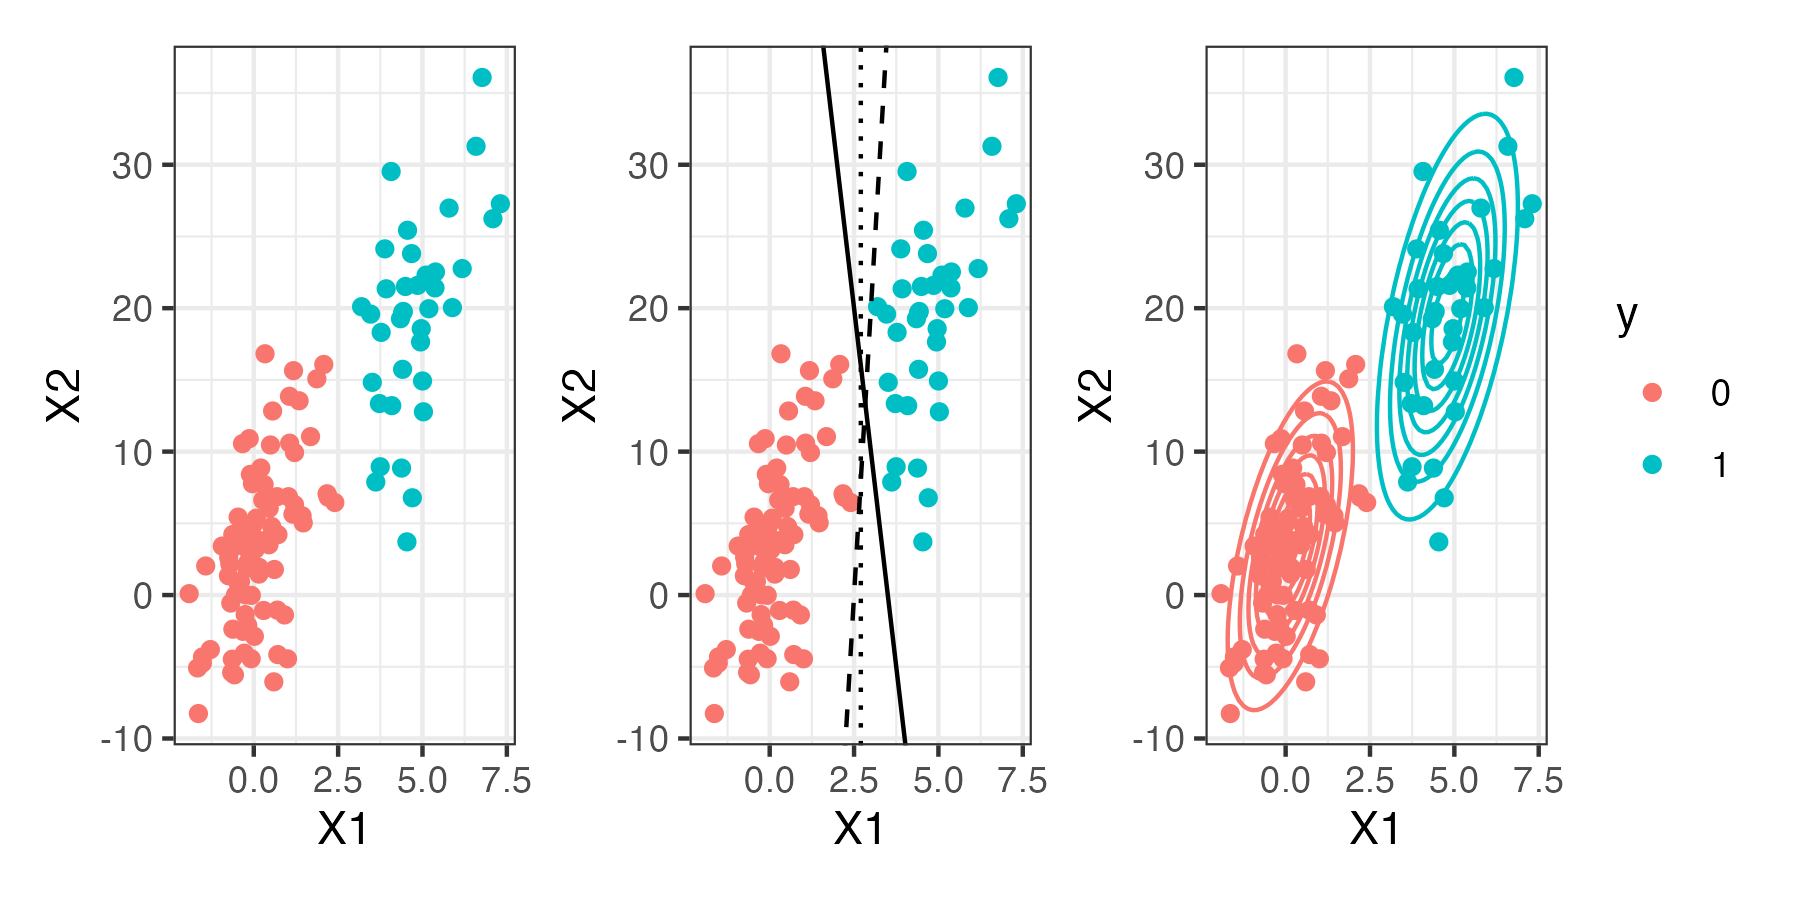
\includegraphics[width=\textwidth]{442_lecs/svm_raw.png}
\caption{A figure to motivate SVMs, and their differences with logistic regression, LDA, or QDA.}
\label{fig_svm}
\end{figure}

What if we want a way to pick between all of the lines in the center panel of Figure~\ref{fig_svm}? And we want a way that does not make a Gaussian assumption, or arbitrarily restrict itself to straight lines defined by a single variable? This is the idea of the maximum margin classifier, which is summarized in Figure~\ref{fig_svm2}, which is taken from ISL. The idea is quite simple: let's pick between all of the possible separating lines by choosing the one that is as far as possible from all of the training observations. 

\begin{figure}
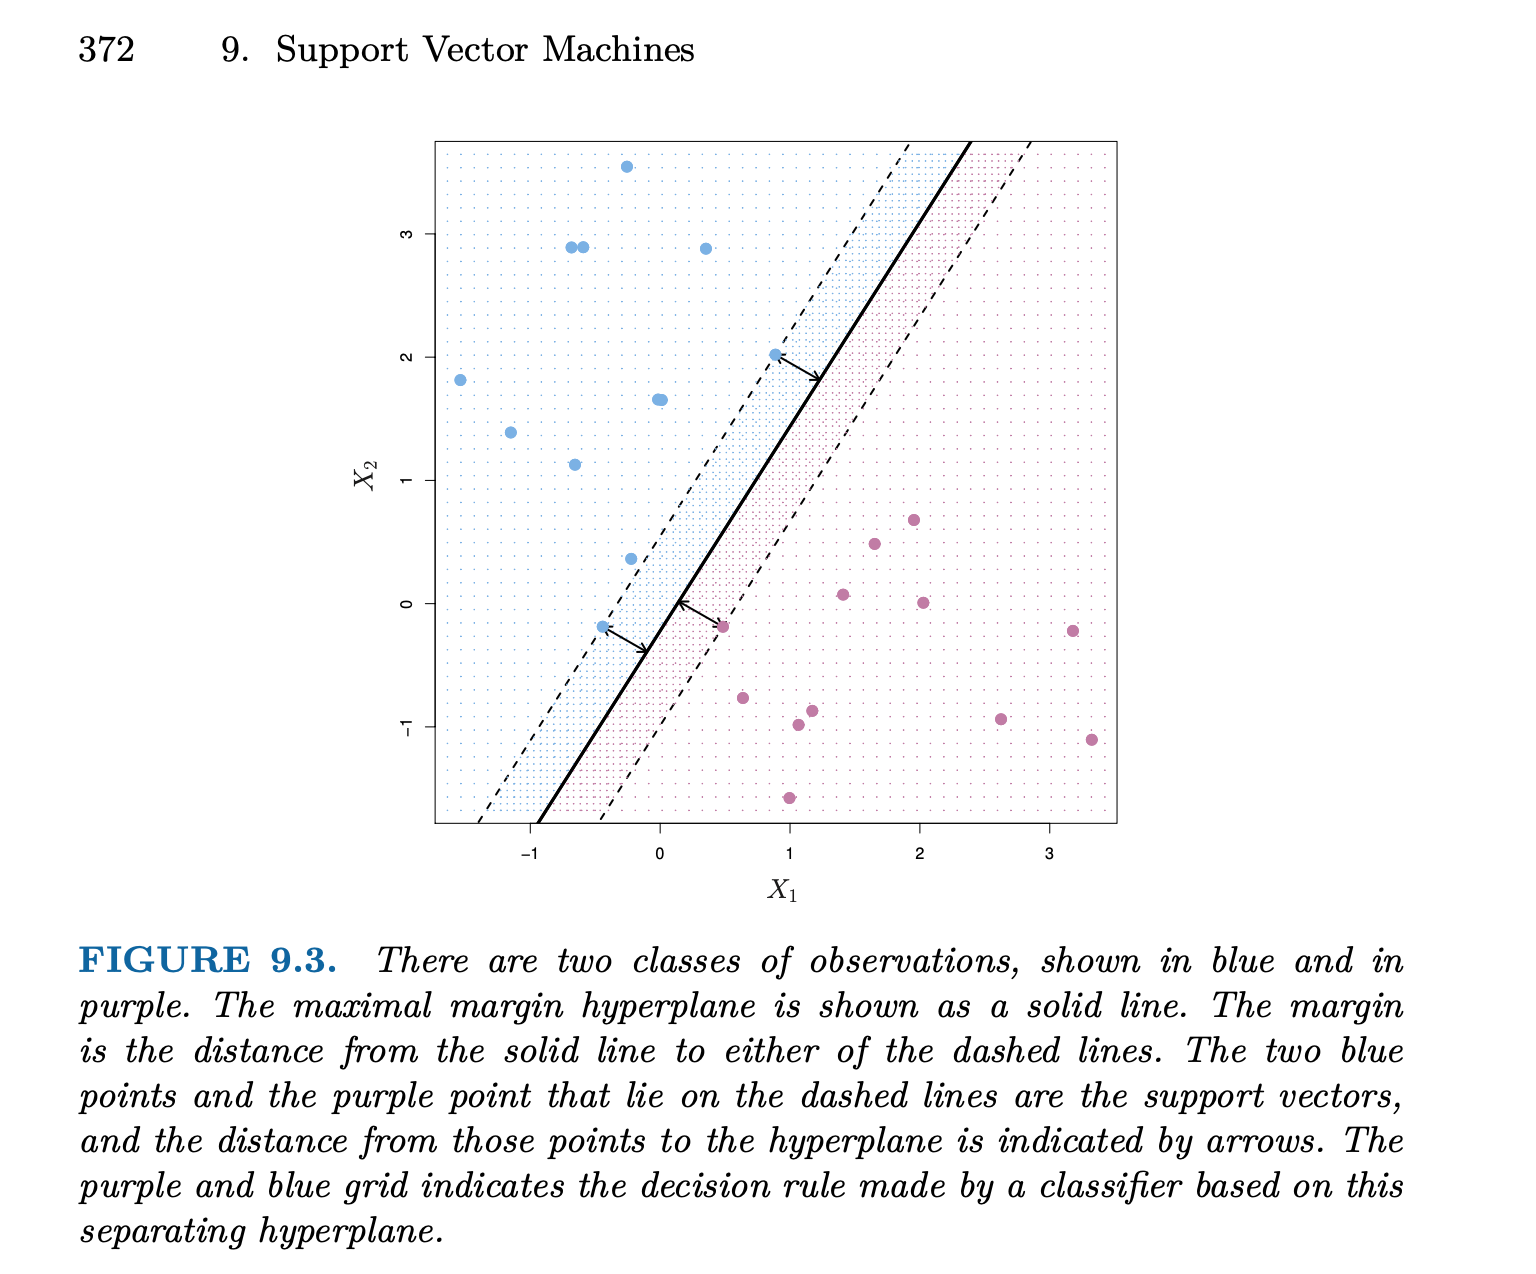
\includegraphics[width=0.8\textwidth]{442_lecs/svm.png}
\caption{The maximum margin classifier picks the line that is far as possible from all observations.}
\label{fig_svm2}
\end{figure}

\subsection{Maximum margin classifier using constrained optimization}

How do we actually fit the line in Figure~\ref{fig_svm2}? There is some math that relates to how we actually draw these lines onto plots. Also, note that we could have more than $2$ $X$ variables, and then we would be using a plane and not a line to separate our classes. 

In general, we will write our linear boundary as the line:
$$
\beta_0 + \beta_1 X_1 + \ldots + \beta_p X_p = 0. 
$$
The idea is to pick a line so that $\beta_0 + \beta_1 X_1 + \ldots + \beta_p X_p < 0$ whenever $y=-1$ and $\beta_0 + \beta_1 X_1 + \ldots + \beta_p X_p > 0$ whenever $y=1$. For today, we are doing binary classification and we are writing our two classes as $-1$ and $1$, for simplicity. 

Any of the lines in the center panel of Figure~\ref{fig_svm} actually have this property. So now the idea is to do even better. Let's both have it be the case that $\beta_0 + \beta_1 X_1 + \ldots + \beta_p X_p < 0$ whenever $y=-1$ and $\beta_0 + \beta_1 X_1 + \ldots + \beta_p X_p > 0$ whenever $y=1$, but also have it be the case that $\beta_0 + \beta_1 X_1 + \ldots + \beta_p X_p$ is basically never TOO close to $0$. Because when it is near $0$, it means that points are close to the line and we have uncertainty. If all of our points are far from the boundary, we have less uncertainty.

One quick note about these hyperplanes: if our class boundary is the line $\beta_0 + \beta_1 X_1 + \ldots + \beta_p X_p = 0$, then $c(\beta_0 + \beta_1 X_1 + \ldots + \beta_p X_p) = 0$ defines the same class boundary for any constant $c$. Thus, in defining planes, we restrict our attention to $\beta$ vectors where $||\beta||_2^2=1$: to make sure that we have a unique solution. 

So, the maximum margin classifier says:

\begin{align*}
&\underset{{\beta_0, \beta_1, \ldots, \beta_p, M}}{\mathrm{maximize}} M \\
&\text{subject to } \sum_{j=1}^p \beta_j^2 = 1 \\
&\text{and } y_i (\beta_0 + \beta_1 x_{i1} + \ldots + \beta_p x_{ip} ) \geq M. 
\end{align*}
The first constraint is just for uniqueness. The second constraint says that every training observation is correctly classified (if M is positive), and the fact that we are maximizing $M$ says that we are trying to make all of our prediction values far from $0$ (recall that $y_i$ is just $-1$ or $1$). 

For your purposes: know that people are good at convex constrained optimization. So this can be solved if the classes are linearly separable: i.e. if a separating hyperplane exists! 

There are actually a few interesting properties of this solution. One interesting property is that the optimal hyperplane actually depends on the data ONLY through the points that lie ON the margin $M$: the other points do not contribute to the $\beta$s at all. In Figure~\ref{fig_svm2}, there are only 3 of these ``support vectors" that actually impact our classifier. That is interesting--- we could add 1,000 blue points to Figure~\ref{fig_svm2}, and as long as we add them on the "blue side" of the current hyperplane, our solution does not change at all. This is interesting!! And is certainly different than LDA-- in LDA, the overall class proportions affect our decision boundary (via the prior). 

You might be worried that this property of SVMs- that they only depend on a few observations- could lead to overfitting. I am certainly worried about that! We usually do not want ONE datapoint to impact our entire classifier that much!

The question you should definitely be asking yourself right now is: what if our classes overlap? Real data never looks like Figure~\ref{fig_svm}. How do we use an SVM in this case? To answer this question, we will discuss two concepts.
\begin{itemize}
\item Concept 1: we can rephrase our optimization problem to allow a small number of mistakes. (this will actually also help with the overfitting concern, even when our classes are technically separable). 
\item Concept 2: if we transform our feature space enough, we can probably make the class linearly separable in new feature space. 
\end{itemize}

We will discuss both of these!

\subsection{Support vector classifier}

The support vector classifier just takes the maximum margin classifier and says ``let's be okay with a few mistakes" (concept 1). 

We once again write a constrained optimization problem, and once again smart people know how to solve it efficiently because it is convex.
\begin{align*}
&\underset{{\beta_0, \beta_1, \ldots, \beta_p, \epsilon_1, \ldots, \epsilon_n, M}}{\mathrm{maximize}} M \\
&\text{subject to } \sum_{j=1}^p \beta_j^2 = 1 \\
&\text{and } y_i (\beta_0 + \beta_1 x_{i1} + \ldots + \beta_p x_{ip} ) \geq M (1-\epsilon_i) \\ 
&\text{and } \epsilon_i \geq 0, \sum_{i=1}^n \epsilon_i \leq C. 
\end{align*} 
The only thing that we added here is that a training datapoint is allowed to be on the ``inside of the margin" ($0 < \epsilon_i < 1$), or even on the wrong side of the hyperplane ($\epsilon_i > 1$). But, we limit how many of these points are allowed using the total cost $C$, which is something that we pick. We still make predictions based on whether or not $\beta_0 + \beta_1 x_{1} + \ldots + \beta_p x_{p}$ is greater than or less than $0$: we just know that there are some mistakes in our training set. 

We usually pick $C$ with cross validation. A large $C$ leads to a cross validation with more bias but less variance. Because, when $C$ is big, we let lots of individual datapoints have non-zero $\epsilon$, which means we let them ``break our rules". This lessens the dependence of the classifier on the individual observations, which means less overfitting and less variance. 

Once again, it turns out that ONLY datapoints with non-zero $\epsilon$ affect the final classifier. If you remove other points, or add other points that fall outside of the margin on the correct side, you do not change the classifier! The observations that DO affect the classifier are called the support vectors. When $C$ is big: we have a LOT of support vectors. So we depend on a LOT of the data-- low variance! When $C$ is small: there are only a few support vectors --- we fit the data really well but we have high variance! 

Overall though, we are still only focusing on observations that are near the boundary. Points that are very clearly members of one class or the other do not affect our classifier rule! This makes it more like logistic regression than LDA. 

\subsection{Support vector machine}

If our data are not linearly separable, we could just make our cost $C$ really big until we end up with a valid classifier. But ... sometimes a hyperplane in our original feature space is simply not going to give us a good rule!

If the relationship between our predictors and our classes is not linear, we should not try to use a separating hyperplane! But the key insight of a support vector machine is that maybe we can use a separating hyperplane in a new feature space. This is exactly the same idea as just 



\subsection{The kernel trick}


\subsection{What do we think about SVMs?}







